\documentclass[12pt, a4paper]{article}
\usepackage{../../../myconfig} % Gọi file cấu hình từ ngoài gốc vào

% ==========================================
% BẮT ĐẦU NỘI DUNG TÀI LIỆU
% ==========================================
\begin{document}

% Truyền 3 tham số: {Nhãn cam} {Chữ to chính giữa} {Chữ ở góc phải Header}
\titlebox{Chủ đề: định kì}{Đề kiểm tra định kì lần 3}{Đề định kì}

\textit{\textbf{Phần I: Thí sinh trả lời từ câu 1 đến câu 12, mỗi câu thí sinh chỉ chọn một phương án}}

\vspace{0.5cm}


% --- CÂU 1 ---
\questionLinesManual{0}{1}{Hàm số nào dưới đây đồng biến trên khoảng \((-\infty; +\infty)\)?}{%
    \begin{tasks}(4)
        \task \(y = x^4 + 3x^2\)
        \task \(y = \dfrac{x - 2}{x + 1}\)
        \task \(y = 3x^3 + 3x - 2\)
        \task \(y = 2x^3 - 5x + 1\)
    \end{tasks}
}

% --- CÂU 2 ---
\questionLinesManual{0}{2}{Giá trị nhỏ nhất của hàm số \( f(x) = x + \dfrac{1}{x} \) trên nửa khoảng \([2; +\infty)\) là:}{%
    \begin{tasks}(4)
        \task 2
        \task \(\dfrac{5}{2}\)
        \task 0
        \task \(\dfrac{7}{2}\)
    \end{tasks}
}

% --- CÂU 3 ---
\questionLinesManual{0}{3}{Biết hàm số \( y = \dfrac{x + a}{x + 1} \) (\( a \) là số thực cho trước, \( a \neq 1 \)) có đồ thị như hình bên. Mệnh đề nào dưới đây đúng?

\begin{center}
\begin{tikzpicture}[scale=0.8, >=latex]
    % Giới hạn vùng hiển thị bằng lệnh \clip
    \clip (-5, -3) rectangle (5, 4);

    % 1. Trục tọa độ Ox, Oy
    \draw[->, black] (-5, 0) -- (5, 0) node[below left, black] {$x$};
    \draw[->, black] (0, -3) -- (0, 4) node[below right, black] {$y$};

    % Gốc tọa độ O
    \node[below left] at (0, 0) {$O$};

    % 2. Các đường tiệm cận (màu xanh dương)
    % Tiệm cận đứng x = -1
    \draw[black] (-1, -3) -- (-1, 4);

    % Tiệm cận ngang y = 1
    \draw[black] (-5, 1) -- (5, 1);

    % 3. Đồ thị hàm số y = (x - 2) / (x + 1)
    % Nhánh bên trái tiệm cận đứng (x < -1)
    \draw[very thick, smooth, domain=-5:-1.05, samples=150] 
        plot (\x, {(\x - 1)/(\x + 1)});

    % Nhánh bên phải tiệm cận đứng (x > -1)
    \draw[very thick, smooth, domain=-0.95:5, samples=150] 
        plot (\x, {(\x - 1)/(\x + 1)});
\end{tikzpicture}
\end{center}
}{%
    \begin{tasks}(4)
        \task \( y' < 0, \, \forall x \neq -1 \)
        \task \( y' > 0, \, \forall x \neq -1 \)
        \task \( y' < 0, \, \forall x \in \mathbb{R} \)
        \task \( y' > 0, \, \forall x \in \mathbb{R} \)
    \end{tasks}
}

% --- CÂU 4 ---
\questionLinesManual{0}{4}{Cho góc \( \alpha \) thỏa \( \cot \alpha = \dfrac{3}{4} \) và \( 0^\circ < \alpha < 90^\circ \). Khẳng định nào sau đây đúng?}{%
    \begin{tasks}(4)
        \task \( \cos \alpha = \dfrac{4}{5} \)
        \task \( \sin \alpha = \dfrac{4}{5} \)
        \task \( \sin \alpha = -\dfrac{4}{5} \)
        \task \( \cos \alpha = -\dfrac{4}{5} \)
    \end{tasks}
}

% --- CÂU 5 ---
\questionLinesManual{0}{5}{Cho cấp số cộng \((u_n)\) có \(u_1 = -2\) và công sai \(d = 3\). Tìm số hạng tổng quát \(u_n\) của cấp số cộng đó.}{%
    \begin{tasks}(4)
        \task \(u_n = 3n + 5\)
        \task \(u_n = 3n - 5\)
        \task \(u_n = 3n - 1\)
        \task \(u_n = 3n + 1\)
    \end{tasks}
}

% --- CÂU 6 ---
\questionLinesManual{0}{6}{Cho hình phẳng \( (H) \) giới hạn bởi các đường \( y = x^2 - 2x - 1 \), \( y = 2x - 4 \). Diện tích hình phẳng giới hạn bởi hình \( (H) \) bằng}{%
    \begin{tasks}(4)
        \task \( \dfrac{2}{3} \)
        \task \( \dfrac{4}{3} \)
        \task \( \dfrac{8}{3} \)
        \task 4
    \end{tasks}
}

% --- CÂU 7 ---
\questionLinesManual{0}{7}{Cho \( \log_2 a = 5, \log_2 b = 7; a, b > 0 \). Giá trị của \( \log_2 (a^2 b^3) \) bằng}{%
    \begin{tasks}(4)
        \task 12
        \task 31
        \task 35
        \task 13
    \end{tasks}
}

% --- CÂU 8 ---
\questionLinesManual{0}{8}{Cho \( F(x) \) là một nguyên hàm của hàm số \( f(x) = \dfrac{1}{x-2} \), biết \( F(1) = 2 \). Giá trị của \( F(0) \) bằng}{%
    \begin{tasks}(4)
        \task \( 2 + \ln 2 \)
        \task \( \ln 2 \)
        \task \( 2 + \ln(-2) \)
        \task \( \ln(-2) \)
    \end{tasks}
}

% --- CÂU 9 ---
\questionLinesManual{0}{9}{Hàm số nào sau đây có một tiệm cận?}{%
    \begin{tasks}(4)
        \task \( y = \dfrac{x+3}{2x-1} \)
        \task \( y = \dfrac{x^2 + 3x - 2}{x+3} \)
        \task \( y = \dfrac{4}{x-1} \)
        \task \( y = \dfrac{2x}{x^2 + 1} \)
    \end{tasks}
}

% --- CÂU 10 ---
\questionLinesManual{0}{10}{Biết \( I = \displaystyle\int_{-1}^{0} \dfrac{3x^2 + 5x - 1}{x - 2} dx = a \ln \dfrac{2}{3} + b, (a, b \in \mathbb{R}). \) Khi đó giá trị của \( a + 4b \) bằng}{%
    \begin{tasks}(4)
        \task 50
        \task 60
        \task 59
        \task 40
    \end{tasks}
}

% --- CÂU 11 ---
\questionLinesManual{0}{11}{Cho hàm số \( y = ax^3 + bx^2 + cx + d \) có đồ thị như hình vẽ bên. Mệnh đề nào dưới đây đúng?

\begin{center}
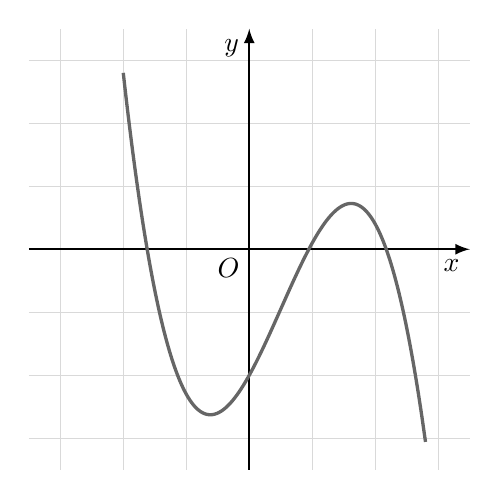
\begin{tikzpicture}[scale=0.8, >=latex]

    % 1. Lưới ô vuông
    \draw[gray!30, thin] (-3.5, -3.5) grid (3.5, 3.5);

    % 2. Trục tọa độ Ox, Oy
    \draw[->, thick] (-3.5, 0) -- (3.5, 0) node[below left] {$x$};
    \draw[->, thick] (0, -3.5) -- (0, 3.5) node[below left] {$y$};

    % Gốc tọa độ O
    \node[below left] at (0, 0) {$O$};

    % 3. Đồ thị hàm số bậc ba y = f(x) = -0.6*x^3 + 0.9*x^2 + 1.8*x - 2
    % Cực tiểu tại x ≈ -0.62 (y ≈ -2.57) nằm bên trái Oy, bên dưới Ox
    % Cắt Oy tại (0, -2) < 0
    % Cực đại tại x ≈ 1.62 (y ≈ 3.7) nằm bên phải Oy, bên trên Ox
    % Nhánh bên phải đi xuống (a < 0)
    \draw[very thick, gray!80!black, smooth, domain=-2:2.8, samples=200] 
        plot (\x, {-0.6*\x*\x*\x + 0.9*\x*\x + 1.8*\x - 2});

\end{tikzpicture}
\end{center}
}{%
    \begin{tasks}(2)
        \task \( a < 0, \, b > 0, \, c > 0, \, d < 0 \)
        \task \( a < 0, \, b < 0, \, c > 0, \, d < 0 \)
        \task \( a > 0, \, b < 0, \, c < 0, \, d > 0 \)
        \task \( a < 0, \, b > 0, \, c < 0, \, d < 0 \)
    \end{tasks}
}


% --- CÂU 12 ---
\questionLinesManual{0}{12}{Cho \( \displaystyle\int_{-2}^{2} f(x) dx = 1, \displaystyle\int_{-2}^{4} f(t) dt = -4 \). Tính \( \displaystyle\int_{2}^{4} f(y) dy \).}{%
    \begin{tasks}(4)
        \task \( I = 5 \)
        \task \( I = -3 \)
        \task \( I = 3 \)
        \task \( I = -5 \)
    \end{tasks}
}

\textit{\textbf{Phần II: Thí sinh trả lời từ câu 13 đến câu 16; trong mỗi ý a), b), c), d) ở mỗi câu, thí sinh chọn đúng hoặc sai.}}

\vspace{0.3cm}


\questionTrueFalse{0}{13}{Cho hàm số  
\( y = ax + b + \dfrac{c}{x + d} \quad (a, b, c, d \in \mathbb{R}) \) 
có đồ thị như hình vẽ sau:

\begin{center}
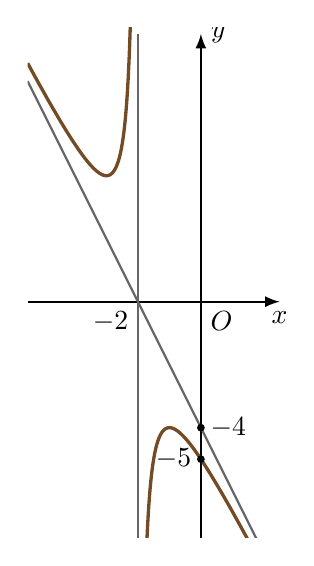
\begin{tikzpicture}[scale=0.4, >=latex]
    % Giới hạn vùng hiển thị bằng \clip
    \clip (-5.5, -7.5) rectangle (2.7, 8.7);

    % 1. Trục tọa độ Ox, Oy
    \draw[->, thick] (-5.5, 0) -- (2.5, 0) node[below] {$x$};
    \draw[->, thick] (0, -7.5) -- (0, 8.5) node[right] {$y$};
    \node[below right] at (0, 0) {$O$};

    % 2. Tiệm cận đứng x = -2
    \draw[thick, gray!80!black] (-2, -7.5) -- (-2, 8.5);

    % 3. Tiệm cận xiên y = -2x - 4
    \draw[thick, gray!80!black, domain=-5.5:2.5, samples=2] plot (\x, {-2*\x - 4});

    % 4. Hai nhánh đồ thị y = -2x - 4 - 2/(x+2)
    % Nhánh bên trái tiệm cận đứng (x < -2)
    \draw[very thick, brown!60!black, smooth, domain=-5.5:-2.2, samples=100] 
        plot (\x, {-2*\x - 4 - 2/(\x + 2)});

    % Nhánh bên phải tiệm cận đứng (x > -2)
    \draw[very thick, brown!60!black, smooth, domain=-1.8:1.5, samples=100] 
        plot (\x, {-2*\x - 4 - 2/(\x + 2)});

    % 5. Đánh dấu các điểm mốc và nhãn số
    \node[below left] at (-2, 0) {$-2$};
    \fill[black] (0, -4) circle (3.5pt) node[right] {$-4$};
    \fill[black] (0, -5) circle (3.5pt) node[left] {$-5$};

\end{tikzpicture}
\end{center}
}{
    \textbf{a)} & Đồ thị hàm số đã cho có tiệm cận đứng là đường thẳng \( x = -2 \).
    & \textcolor{amberorange}{$\bigcirc$} & \textcolor{amberorange}{$\bigcirc$} \\ \hline
    
    \textbf{b)} & Giá trị \( b = -4 \).
    & \textcolor{amberorange}{$\bigcirc$} & \textcolor{amberorange}{$\bigcirc$} \\ \hline
    
    \textbf{c)} & Đồ thị hàm số đã cho có tiệm cận xiên là đường thẳng \( y = 2x - 4 \).
    & \textcolor{amberorange}{$\bigcirc$} & \textcolor{amberorange}{$\bigcirc$} \\ \hline
    
    \textbf{d)} & Hàm số đã cho là \( y = -2x - 4 - \dfrac{2}{x + 2} \).
    & \textcolor{amberorange}{$\bigcirc$} & \textcolor{amberorange}{$\bigcirc$} \\
}


\questionTrueFalse{0}{14}{Cho đồ thị hàm số \( C: y = x^3 - 2x^2 - 3x + 4 \). Đường thẳng \( d: y = 2x - 2 \) cắt đồ thị \( C \) thành 2 miền có diện tích là \( S_1 \) và \( S_2 \) như hình vẽ.

\begin{center}
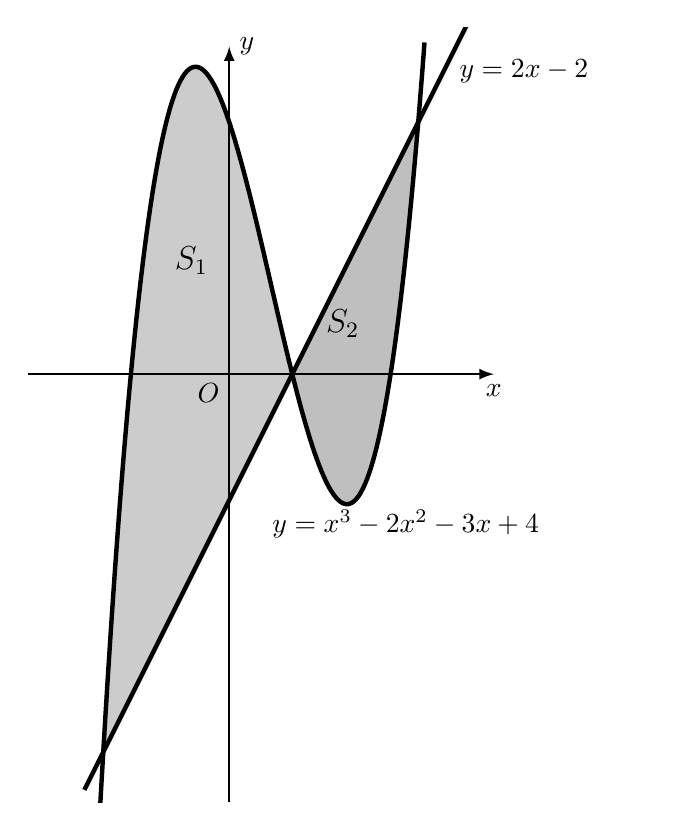
\begin{tikzpicture}[scale=0.8, >=latex]
    % Giới hạn vùng hiển thị bằng \clip
    \clip (-3.2, -6.8) rectangle (7, 5.5);

    % 1. Tô màu các miền diện tích S1 và S2
    % Miền S1: từ x = -2 đến x = 1 (Đồ thị C ở trên, đường d ở dưới)
    \fill[gray!40] plot[domain=-2:1, samples=100] (\x, {\x*\x*\x - 2*\x*\x - 3*\x + 4}) 
        -- plot[domain=1:-2, samples=100] (\x, {2*\x - 2}) -- cycle;

    % Miền S2: từ x = 1 đến x = 3 (Đường d ở trên, đồ thị C ở dưới)
    \fill[gray!50] plot[domain=1:3, samples=100] (\x, {2*\x - 2}) 
        -- plot[domain=3:1, samples=100] (\x, {\x*\x*\x - 2*\x*\x - 3*\x + 4}) -- cycle;

    % 2. Hệ trục tọa độ Ox, Oy
    \draw[->, thick] (-3.2, 0) -- (4.2, 0) node[below] {$x$};
    \draw[->, thick] (0, -6.8) -- (0, 5.2) node[right] {$y$};
    \node[below left] at (0, 0) {$O$};

    % 3. Đồ thị hàm số bậc ba (C): y = x^3 - 2x^2 - 3x + 4
    \draw[ultra thick, black, domain=-2.1:3.1, samples=150] 
        plot (\x, {\x*\x*\x - 2*\x*\x - 3*\x + 4});

    % 4. Đường thẳng d: y = 2x - 2
    \draw[ultra thick, black, domain=-2.3:3.8, samples=2] plot (\x, {2*\x - 2});

    % 5. Nhãn các miền và tên hàm số
    \node[font=\large] at (-0.6, 1.8) {$S_1$};
    \node[font=\large] at (1.8, 0.8) {$S_2$};

    \node[right] at (3.5, 4.8) {$y = 2x - 2$};
    \node[below] at (2.8, -2) {$y = x^3 - 2x^2 - 3x + 4$};

\end{tikzpicture}
\end{center}
}{
    \textbf{a)} & Diện tích hình phẳng giới hạn bởi đồ thị \( C \) và đường thẳng \( d \) bằng \(\dfrac{253}{12}\).
    & \textcolor{amberorange}{$\bigcirc$} & \textcolor{amberorange}{$\bigcirc$} \\ \hline
    
    \textbf{b)} & Đường thẳng \( d \) cắt \( C \) tại ba điểm phân biệt \( A(-2; -6); B(1; 0); C(3; 4) \).
    & \textcolor{amberorange}{$\bigcirc$} & \textcolor{amberorange}{$\bigcirc$} \\ \hline
    
    \textbf{c)} & Diện tích hình phẳng giới hạn bởi đồ thị \( C, Ox \) và đường thẳng \( x = -1; x = 2 \) bằng \(\dfrac{21}{4}\).
    & \textcolor{amberorange}{$\bigcirc$} & \textcolor{amberorange}{$\bigcirc$} \\ \hline
    
    \textbf{d)} & Tỉ số \(\dfrac{S_1}{S_2} = \dfrac{63}{16}\).
    & \textcolor{amberorange}{$\bigcirc$} & \textcolor{amberorange}{$\bigcirc$} \\
}

\questionTrueFalse{0}{15}{Khối chỏm cầu có bán kính \( R = 10 \) và chiều cao \( h = 8 \) sinh ra khi quay hình phẳng giới hạn bởi cung tròn có phương trình \( y = \sqrt{100 - x^2} \), trục hoành và hai đường thẳng \( x = 2, x = 10 \) xung quanh trục \( Ox \).

\begin{center}
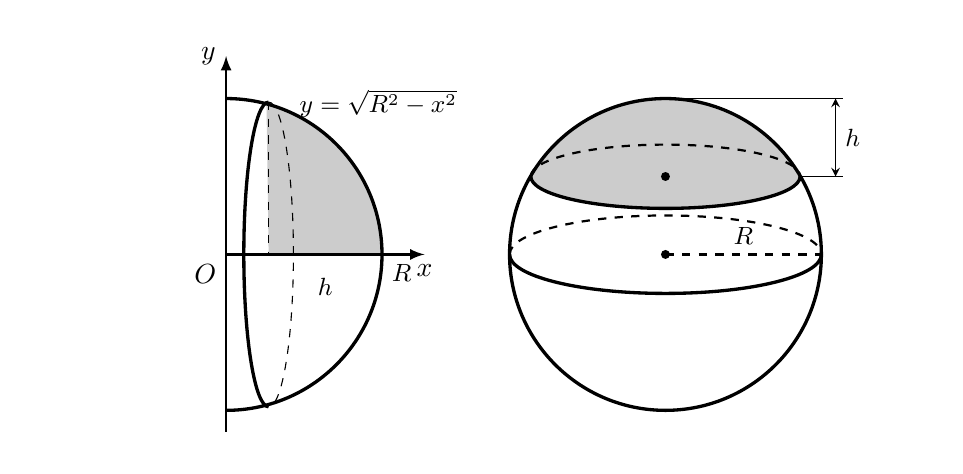
\begin{tikzpicture}[scale=0.9, >=latex]
    % Giới hạn vùng hiển thị bằng \clip
    \clip (-2.8, -2.7) rectangle (10.0, 3.2);

    % ==================== HÌNH 1: HỆ TRỤC Oxyz & CHỎM CẦU TRÒN XOAY ====================
    \begin{scope}[shift={(0,0)}]
        % 1. Tô màu phần chỏm cầu (miền xám)
        \fill[gray!40] (0.6, 0) -- (2.2, 0) 
            arc [start angle=0, end angle=75, radius=2.2] 
            -- cycle;

        % 2. Các trục tọa độ
        \draw[->, thick] (0, 0) -- (2.8, 0) node[below] {$x$};
        \draw[->, thick] (0, -2.5) -- (0, 2.8) node[left] {$y$};
        \node[below left] at (0, 0) {$O$};

        % 3. Cung tròn nửa cầu y = sqrt(R^2 - x^2)
        \draw[very thick] (0, 2.2) arc (90:-90:2.2);

        % 4. Mặt đáy chỏm cầu: Nửa sau NÉT ĐỨT, nửa trước NÉT LIỀN
        \draw[very thick] (0.6, 2.15) arc [start angle=90, end angle=270, x radius=0.35, y radius=2.15];
        \draw[dashed] (0.6, 2.15) arc [start angle=90, end angle=-90, x radius=0.35, y radius=2.15];
        \draw[dashed] (0.6, 2.15)-- (0.6,0);

        \node[below, font=\small] at (1.4, -0.2) {$h$};

        % Điểm R
        \node[below right, font=\small] at (2.2, 0) {$R$};

        % Nhãn phương trình
        \node[above right, font=\small] at (0.9, 1.8) {$y = \sqrt{R^2 - x^2}$};
    \end{scope}

    % ==================== HÌNH 2: KHỐI CẦU VÀ CHỎM CẦU ====================
    % Đã tăng khoảng cách x (shift={(6.2,0)}) để 2 hình xa nhau hơn
    \begin{scope}[shift={(6.2,0)}]
        % 1. Tô màu phần chỏm cầu bên trên
        \fill[gray!40] (0, 1.1) ellipse (1.9cm and 0.45cm);
        \fill[gray!40] (-1.9, 1.1) arc [start angle=150, end angle=30, radius=2.2] -- cycle;

        % 2. Mặt cầu bên ngoài
        \draw[very thick] (0,0) circle (2.2cm);

        % 3. Đường xích đạo: Nửa sau NÉT ĐỨT, nửa trước NÉT LIỀN
        \draw[thick, dashed] (-2.2, 0) arc [start angle=180, end angle=0, x radius=2.2, y radius=0.55];
        \draw[very thick] (-2.2, 0) arc [start angle=180, end angle=360, x radius=2.2, y radius=0.55];

        % 4. Đáy chỏm cầu: Nửa sau NÉT ĐỨT, nửa trước NÉT LIỀN
        \draw[thick, dashed] (-1.9, 1.1) arc [start angle=180, end angle=0, x radius=1.9, y radius=0.45];
        \draw[very thick] (-1.9, 1.1) arc [start angle=180, end angle=360, x radius=1.9, y radius=0.45];

        % 5. Các điểm tâm
        \fill[black] (0, 0) circle (1.8pt);
        \fill[black] (0, 1.1) circle (1.8pt);

        % 6. Bán kính R (nét đứt từ tâm ra viền phải)
        \draw[thick, dashed] (0,0) -- (2.2,0);
        \node[above, font=\small] at (1.1, 0) {$R$};

        % 7. Kích thước chiều cao h bên phải
        \draw[<->, >=stealth, thin] (2.4, 1.1) -- (2.4, 2.2);
        \draw[thin] (1.9, 1.1) -- (2.5, 1.1);
        \draw[thin] (0, 2.2) -- (2.5, 2.2);
        \node[right, font=\small] at (2.4, 1.65) {$h$};
    \end{scope}

\end{tikzpicture}
\end{center}
}{
    \textbf{a)} & Khoảng cách từ tâm của khối cầu đến khối chỏm cầu bằng 6.
    & \textcolor{amberorange}{$\bigcirc$} & \textcolor{amberorange}{$\bigcirc$} \\ \hline
    
    \textbf{b)} & Thể tích của khối chỏm cầu \( V_1 \) được tính theo công thức  
    \(V_1 = \pi \displaystyle\int_{0}^{10} \left( \sqrt{100 - x^2} \right) dx.\)
    & \textcolor{amberorange}{$\bigcirc$} & \textcolor{amberorange}{$\bigcirc$} \\ \hline
    
    \textbf{c)} & Thể tích của khối chỏm cầu \( V_1 = \dfrac{112\pi}{3} \).
    & \textcolor{amberorange}{$\bigcirc$} & \textcolor{amberorange}{$\bigcirc$} \\ \hline
    
    \textbf{d)} & Gọi \( V_2 \) là thể tích của nửa khối cầu có bán kính bằng 6. Tỉ số thể tích \( \dfrac{V_1}{V_2} = \dfrac{7}{27} \).
    & \textcolor{amberorange}{$\bigcirc$} & \textcolor{amberorange}{$\bigcirc$} \\
}

\questionTrueFalse{0}{16}{Một trang trại cần xây một bể chứa nước hình trụ bằng bê tông (có nắp đậy) để chứa \( 60(m^3) \) nước tưới tiêu. Chi phí xây dựng chủ yếu phụ thuộc vào diện tích bề mặt bê tông cần sử dụng (diện tích toàn phần của bể tính theo phần bên trong của bể). Theo hợp đồng với nhà thầu xây dựng, chi phí mỗi mét vuông xây dựng theo cách tính trên là 1,5 triệu đồng. Gọi \( r \) là bán kính đáy và \( h \) là chiều cao của bể (đơn vị tính của \( r, h \) là mét).
\begin{figure}[H]
    \centering
    
\includegraphics[width=0.4\textwidth]{images/trunuoc.png}
\end{figure}

}{
    \textbf{a)} & Thể tích của bể là: \(V = \pi r^2 h = 60(m^3)\).
    & \textcolor{amberorange}{$\bigcirc$} & \textcolor{amberorange}{$\bigcirc$} \\ \hline
    
    \textbf{b)} & Diện tích toàn phần \( S_{tp} \) của bể chứa nước được biểu diễn theo bán kính \( r \) là  
    \(S_{tp}(r) = \pi r^2 + \dfrac{120}{r}(m^2)\).
    & \textcolor{amberorange}{$\bigcirc$} & \textcolor{amberorange}{$\bigcirc$} \\ \hline
    
    \textbf{c)} & Để tiết kiệm chi phí nhất, bể nên được xây với bán kính đáy là  
    \(r = \sqrt[3]{\dfrac{30}{\pi}}(m)\).
    & \textcolor{amberorange}{$\bigcirc$} & \textcolor{amberorange}{$\bigcirc$} \\ \hline
    
    \textbf{d)} & Chi phí thấp nhất để xây dựng bể chứa nước nói trên là 127 triệu đồng (làm tròn kết quả đến hàng đơn vị).
    & \textcolor{amberorange}{$\bigcirc$} & \textcolor{amberorange}{$\bigcirc$} \\
}

\textit{\textbf{Phần III: Thí sinh trả lời từ câu 17 đến câu 22.}}

\vspace{0.3cm}

\questionShortAnswer{0}{17}{Giả sử số lượng tế bào của một quần thể nấm men tại môi trường nuôi cấy trong phòng thí nghiệm được mô hình hóa bằng hàm số  
\(P(t) = \dfrac{a}{b + e^{-0.75t}}\) (với \(a, b \in \mathbb{R}\)), trong đó thời gian \(t\) được tính bằng giờ. Đạo hàm của hàm số \(y = P(t)\) biểu thị tốc độ sinh trưởng của nấm men (tính bằng tế bào/giờ) tại thời điểm \(t\) (giờ). Tại thời điểm ban đầu \(t = 0\), quần thể có 20 tế bào và tốc độ sinh trưởng là 10 tế bào/giờ. Tìm số lượng tế bào của quần thể nấm men tại thời điểm tốc độ sinh trưởng của quần thể đạt mức tối đa.
}

\questionShortAnswer{0}{18}{Một khu vui chơi giải trí giành cho trẻ em đang có kế hoạch điều chỉnh giá vé để tăng lợi nhuận. Sau khi khảo sát thị trường, người ta xác định được rằng: nếu giá vé vào cửa là 50000/người thì trung bình có 500 người đến. Nhưng nếu tăng thêm 1000/người thì sẽ mất 10 khách hàng hoặc giảm đi 1000/người thì sẽ có thêm 10 khách hàng trong số trung bình. Biết rằng, trung bình, mỗi khách hàng còn đem lại 5000 lợi nhuận trong các dịch vụ đi kèm. Hỏi giá vé vào cửa là bao nhiêu nghìn đồng để thu nhập là lớn nhất?

}

\questionShortAnswer{0}{19}{Khu vườn nhà ông Ba có dạng hình tròn, bán kính 10 m. Ông Ba dự định trồng hoa Hồng ở khu vực \( S_1 \) và hoa Ly ở khu vực hình bán nguyên \( S_2 \). Với \( S_1 \) là phần diện tích giới hạn bởi đường parabol đi qua tâm hình tròn và \( S_2 \) là phần diện tích giới hạn bởi nửa đường elip không chứa tâm hình tròn (kích thước như hình vẽ). Biết rằng kinh phí trồng hoa Hồng là 100.000 đồng/ \( m^2 \), kinh phí trồng hoa Ly là 150.000 đồng/ \( m^2 \). Hỏi ông Ba phải mất bao nhiêu triệu đồng để trồng hoa lên hai khu đất đó (làm tròn kết quả đến hàng phần mười).

\begin{center}
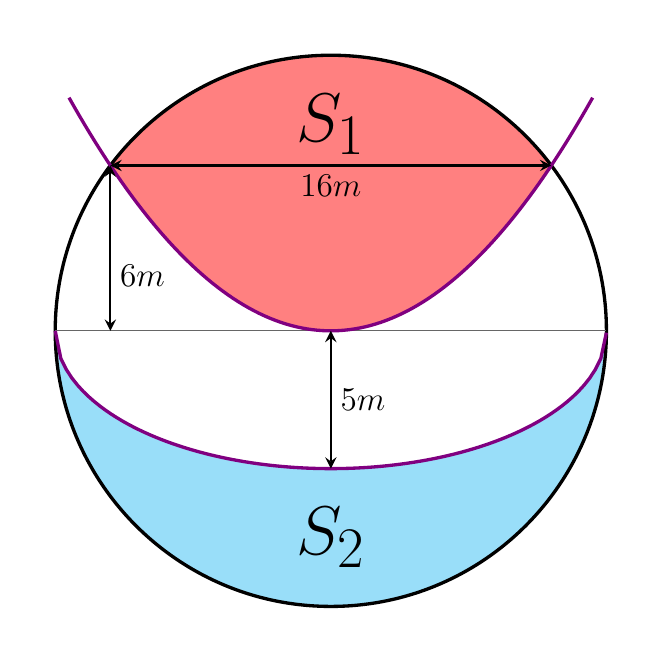
\begin{tikzpicture}[scale=0.35, >=latex]
    % Giới hạn vùng hiển thị bằng \clip
    \clip (-11, -11) rectangle (11, 11);

    % 1. Tô màu các miền S1 và S2
    % Miền S1 (đỏ nhạt)
    \fill[red!50] plot[domain=-8:8, samples=100] (\x, {sqrt(100 - \x*\x)}) 
        -- plot[domain=8:-8, samples=100] (\x, {3/32*\x*\x}) -- cycle;

    % Miền S2 (xanh nhạt)
    \fill[cyan!40] plot[domain=-10:10, samples=100] (\x, {-sqrt(100 - \x*\x)}) 
        -- plot[domain=10:-10, samples=100] (\x, {-0.5*sqrt(100 - \x*\x)}) -- cycle;

    % 2. Đường tròn khu vườn
    \draw[very thick, black] (0,0) circle (10cm);

    % 3. Đường thẳng đường kính ngang
    \draw[thin, black!60] (-10,0) -- (10,0);

    % 4. Parabol chứa S1 (màu tím/xanh đậm)
    \draw[very thick, violet, domain=-9.5:9.5, samples=100] plot (\x, {3/32*\x*\x});

    % 5. Nửa Elip chứa S2 (màu tím/xanh đậm)
    \draw[very thick, violet, domain=-10:10, samples=100] plot (\x, {-0.5*sqrt(100 - \x*\x)});

    % 6. Các đường kích thước và mũi tên
    % Kích thước 16m
    \draw[<->, >=stealth, thick] (-8, 6) -- (8, 6);
    \node[below, font=\large] at (0, 6) {$16\text{m}$};

    % Kích thước 6m
    \draw[<->, >=stealth, thick] (-8, 0) -- (-8, 6);
    \node[right, font=\large] at (-8, 2) {$6\text{m}$};

    % Kích thước 5m
    \draw[<->, >=stealth, thick] (0, 0) -- (0, -5);
    \node[right, font=\large] at (0, -2.5) {$5\text{m}$};

    % 7. Tên các miền S1, S2
    \node[font=\Huge\bfseries] at (0, 7.5) {$S_1$};
    \node[font=\Huge\bfseries] at (0, -7.5) {$S_2$};

\end{tikzpicture}
\end{center}
}

\questionShortAnswer{0}{20}{Sau khi phát hiện một bệnh dịch, các chuyên gia y tế ước tính số người nhiễm bệnh kể từ ngày xuất hiện bệnh nhân đầu tiên đến ngày thứ \( t \) là  
\(f(t) = 180t + 42t^2 - t^3, \, t = 0, 1, \ldots, 30.\)  
Nếu coi \( f(t) \) là hàm số xác định trên đoạn \([0; 30]\) thì đạo hàm \( f'(t) \) được xem là tốc độ truyền bệnh (đơn vị: người/ngày) tại thời điểm \( t \). Hỏi trong 30 ngày đó, có bao nhiêu ngày mà tốc độ truyền bệnh giảm?}

\questionShortAnswer{0}{21}{Một vật trang trí có dạng một khối tròn xoay được tạo thành khi quay miền \( (R) \) (phần được tô màu trong hình vẽ bên) quanh trục \( AB \). Miền \( (R) \) được giới hạn bởi các cạnh \( AB, AD \) của hình vuông \( ABCD \) và các cung phần tư của các đường tròn bán kính bằng 1 cm với tâm lần lượt là trung điểm của các cạnh \( AD, AB \). Tính thể tích của vật trang trí đó, làm tròn kết quả đến hàng phần mười.

\begin{center}
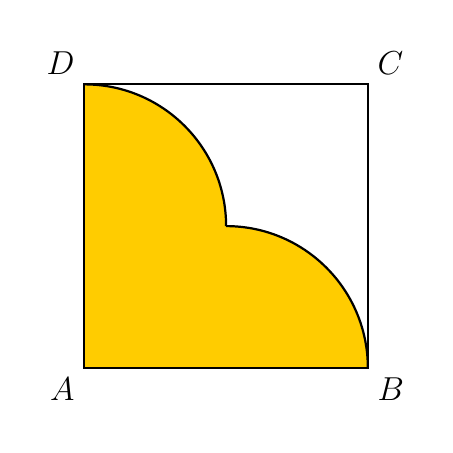
\begin{tikzpicture}[scale=1.8, >=latex]
    % Giới hạn vùng hiển thị bằng \clip
    \clip (-0.4, -0.4) rectangle (2.4, 2.4);

    % 1. Tô màu xám/vàng cho miền (R)
    \fill[orange!40!yellow] (0, 0) -- (0, 2) 
        arc [start angle=90, end angle=0, radius=1] 
        arc [start angle=90, end angle=0, radius=1] 
        -- (0, 0) -- cycle;

    % 2. Khung hình vuông ABCD
    \draw[thick, black] (0, 0) rectangle (2, 2);

    % 3. Cung đường tròn phần tư thứ nhất (tâm (0,1), bán kính 1)
    \draw[thick, black] (0, 2) arc [start angle=90, end angle=0, radius=1];

    % 4. Cung đường tròn phần tư thứ hai (tâm (1,0), bán kính 1)
    \draw[thick, black] (1, 1) arc [start angle=90, end angle=0, radius=1];

    % 5. Tên các đỉnh hình vuông
    \node[below left, font=\large] at (0, 0) {$A$};
    \node[below right, font=\large] at (2, 0) {$B$};
    \node[above right, font=\large] at (2, 2) {$C$};
    \node[above left, font=\large] at (0, 2) {$D$};

\end{tikzpicture}
\end{center}
}

\questionShortAnswer{0}{22}{Một chiếc cổng hình Parabol có chiều cao \( 9 \, m \), khoảng cách giữa hai chân cổng là \( 6 \, m \). Để vận chuyển thùng hàng hình chữ nhật qua cổng, người ta dùng một xe kéo có chiều cao \( 1 \, m \). Biết rằng mặt cắt của thùng hàng qua cổng là hình chữ nhật, hỏi diện tích hình chữ nhật đó lớn nhất là bao nhiêu \( m^2 \) để xe chở thùng hàng có thể đi qua được cổng (kết quả làm tròn đến hàng phần chục).

\begin{figure}[H]
    \centering
    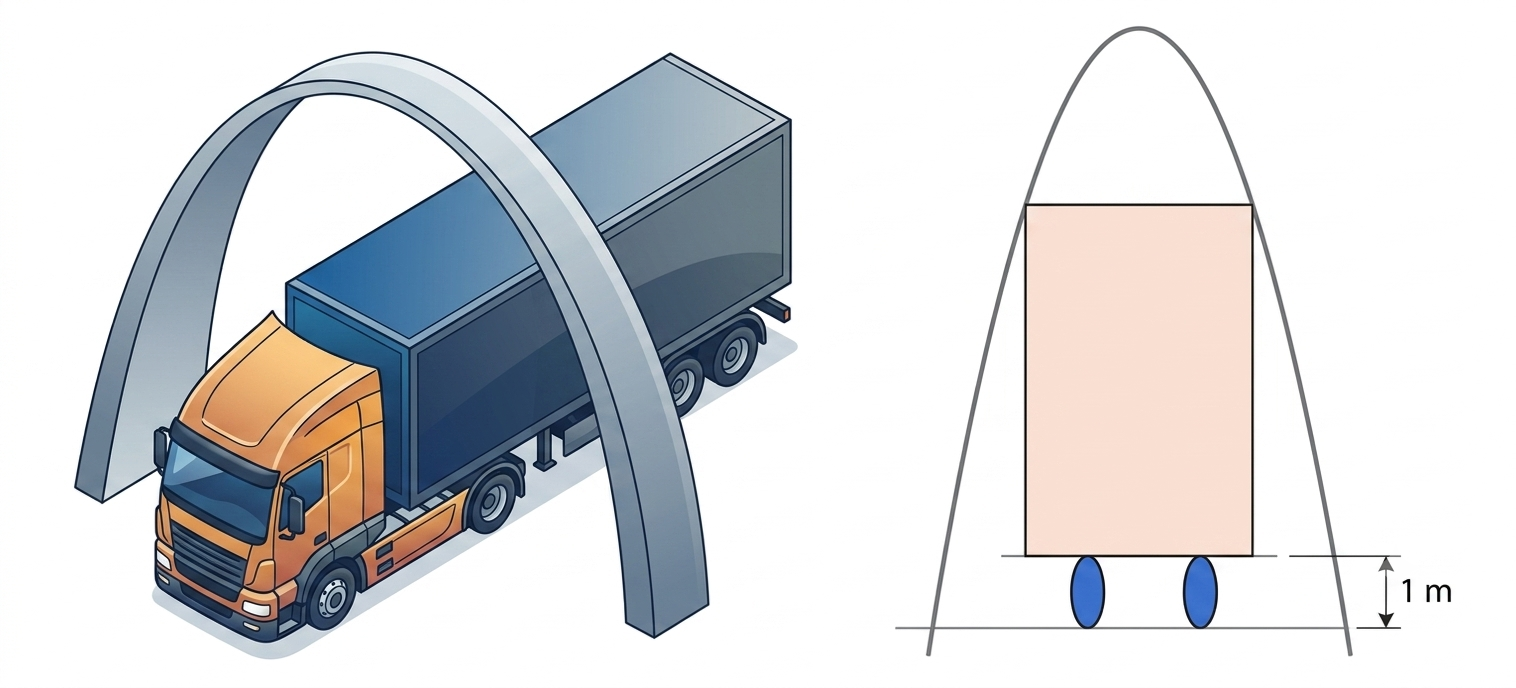
\includegraphics[width=0.6\textwidth]{images/Xetai.png}
\end{figure}

}


\end{document}